\documentclass{beamer}
\usetheme{Montpellier}
\usecolortheme{dolphin}
%% Checking if saving file is working more
%\usepackage{graphicx} %For jpg figure inclusion
%\usepackage{times} %For typeface
%\usepackage{epsfig}
\usepackage{color} %For Comments
\usepackage{beamerthemeshadow} %Paul and Lemmon put this in, take out if you want
%\usepackage[all]{xy}
%\usepackage{float}
%\usepackage{subfigure} 
%\usepackage{hyperref}
%\usepackage{url}
%\usepackage{parskip}
%\usepackage{multirow}

\definecolor{ForestGreen}{RGB}{34,139,34}
\definecolor{BlueViolet}{RGB}{138,43,226}
\definecolor{Coquelicot}{RGB}{255, 56, 0}
\definecolor{Teal}{RGB}{2,132,130}
\definecolor{PrettyBlue}{RGB}{0,0,255}
% Uncomment this if you want to show work-in-progress comments
\newcommand{\comment}[1]{{\bf \tt  {#1}}}
% Uncomment this if you don't want to show comments
%\newcommand{\comment}[1]{}
\newcommand{\emcomment}[1]{\textcolor{ForestGreen}{\comment{Elena: {#1}}}}
\newcommand{\todo}[1]{\textcolor{blue}{\comment{To Do: {#1}}}}
\newcommand{\pscomment}[1]{\textcolor{Coquelicot}{\comment{Paul: {#1}}}}
\newcommand{\mmcomment}[1]{\textcolor{magenta}{\comment{Max: {#1}}}}
\newcommand{\escomment}[1]{\textcolor{BlueViolet}{\comment{Emma: {#1}}}}
\newcommand{\alcomment}[1]{\textcolor{red}{\comment{Lemmon: {#1}}}}
\newcommand{\hfcomment}[1]{\textcolor{Teal}{\comment{Henry: {#1}}}}
%%%%%%%%%%%%%%%%%%%%%%%%%%%%%%%%%%%%%%%%%%

\begin{document}
\title{Improving Clojure Usablilty for Introductory Course}
\date{July 8, 2015}

\begin{frame}
\frametitle {Improving Clojure Usablilty for Introductory Course}
{\centering
\noindent
Henry Fellows, Thomas Hagen, Sean Stockholm, Ryan McArthur, and Elena Machkasova \par

{\it 
Minnesota Clojure Users Group Meeting\par
July 8, 2015\par}
}
\end{frame}
%frame

\begin{frame}
\frametitle{Table of contents}
\tableofcontents  
\end{frame}

\section{Overview of the Project}

\begin{frame}
	\frametitle{Goals}
	\begin{itemize}
		\item Integrate Clojure into an introductory CS class
		\item Currently use Racket
		\begin{itemize}
			\item Limited teaching language
			\item Difficult to make complex projects
			\item Students hitting performance issues (!)
		\end{itemize}
	\end{itemize}
\end{frame}

\begin{frame}
	\frametitle{Why use Clojure?}
	\begin{itemize}
		\item Used in industry
		\item Better on resume
		\item Support for concurrency
		\item Large community and excellent resources
		\item Excellent libraries (data processing, image recognition, graphical, musical)
	\end{itemize}
\end{frame}

\begin{frame}
	\frametitle{Issues with Clojure}
	\begin{itemize}
		\item Confusing error messages
		\item Lack of beginner-friendly graphics libraries in functional style
		\item Some misleading or confusing core functions ({\tt conj, some}, string functions).   
	\end{itemize}
\end{frame}

\section{Error Handling}

\begin{frame}
	\frametitle{Error Messages}
	\begin{itemize}
		\item Computers are literal
		\item Error messages are the only way to communicate when something goes wrong
		\item By the time an error is detected, a lot of the context is lost
	\end{itemize}
\end{frame}

\begin{frame}
	\frametitle{Error Messages for Beginners}
	\begin{itemize}
		\item Use terminology that beginners haven't been introduced to
		\item Beginner mistakes can lead to very complex errors
		\item Beginners don't read error messages
		\item Line number reporting needs to be accurate
		\item Good error messages should lead to a correct fix (study of Racket error messages)
		\item Very little (if any) systematic usability study of error messages
	\end{itemize}
\end{frame}

\begin{frame}
	\frametitle{Clojure Error Messages}
	\begin{itemize}
		\item Java exceptions
		\item Use not only Java types, but Java terminology: "cannot be cast", "null pointer"
		\item Very verbose
		\item Stack traces are long
		\item Compiler messages come with a separate cause
	\end{itemize}
\end{frame}

\begin{frame}[fragile]
\frametitle{Example Clojure Error}
		\begin{verbatim}
		Exception in thread "main" clojure.lang.ArityException:
		Wrong number of args (3) passed to: core/cons, compiling:
		(/tmp/form-init3025539740275626138.clj:1:72)
	at clojure.lang.Compiler.load(Compiler.java:7142)
	at clojure.lang.Compiler.loadFile(Compiler.java:7086)
	at clojure.main$load_script.invoke(main.clj:274)
	at clojure.main$init_opt.invoke(main.clj:279)
	at clojure.main$initialize.invoke(main.clj:307)
	at clojure.main$null_opt.invoke(main.clj:342)
	at clojure.main$main.doInvoke(main.clj:420)
	at clojure.lang.RestFn.invoke(RestFn.java:421)
	at clojure.lang.Var.invoke(Var.java:383)
	at clojure.lang.AFn.applyToHelper(AFn.java:156)
	at clojure.lang.Var.applyTo(Var.java:700)
	at clojure.main.main(main.java:37)
		\end{verbatim}	
\end{frame}



\begin{frame}
	\frametitle{Our Error Messages}
	\begin{itemize}
		\item We are not changing language definition
		\item A combination of two approaches: 
		\begin{itemize}
		\item Approach 1: overwrite common functions ({\tt map, filter, +} to add pre-conditions for precise parameter reporting
		\item Approach 2: catch exceptions, match and replace the error message	
		\end{itemize}
		\item Filter the stack trace
		\item Avoid unfamiliar terminology
		\item Consistency within error messages
		\item Readable and short
		\item Future direction: adding hints for common sources of errors
	\end{itemize}
\end{frame}

\begin{frame}[fragile]
\frametitle{First iteration}
		\begin{verbatim}
Error: Wrong number of arguments (3) passed to a function cons.
Found in file core.clj on line 108 in function -main.
	intro.core/-main (core.clj line 108)
	\end{verbatim}	
\end{frame}

\begin{frame}[fragile]
\frametitle{Current message}
		\begin{verbatim}
Error: You cannot pass three arguments to a function cons, need two.
Found in file core.clj on line 108 in function -main.
	intro.core/-main (core.clj line 108)
	\end{verbatim}	
\end{frame}

\begin{frame}[fragile]
\frametitle{Compilation messages}
	We can handle compiler errors
	\begin{itemize}
	\item Compiler errors are often nested
	\item Many compiler errors in Clojure 1.7.0 were runtime in earlier versions
	\end{itemize}
\end{frame}

\begin{frame}[fragile]
\frametitle{Current message}
	\begin{verbatim}
	Exception in thread "main" java.lang.IllegalArgumentException:
	Parameter declaration "5" should be a vector, compiling:
	(core.clj:104:5)
	at clojure.lang.Compiler.macroexpand1(Compiler.java:6644)
	at clojure.lang.Compiler.analyzeSeq(Compiler.java:6719)
	at clojure.lang.Compiler.analyze(Compiler.java:6524)
	at clojure.lang.Compiler.analyze(Compiler.java:6485)
	at clojure.lang.Compiler$BodyExpr$Parser.parse(Compiler.java:5861)
	at clojure.lang.Compiler$TryExpr$Parser.parse(Compiler.java:2261)
	at clojure.lang.Compiler.analyzeSeq(Compiler.java:6733)
	at clojure.lang.Compiler.analyze(Compiler.java:6524)
	at clojure.lang.Compiler.analyze(Compiler.java:6485)
	at clojure.lang.Compiler$BodyExpr$Parser.parse(Compiler.java:5861)
	at clojure.lang.Compiler$FnMethod.parse(Compiler.java:5296)
	at clojure.lang.Compiler$FnExpr.parse(Compiler.java:3925)
	\end{verbatim}	
\end{frame}

\begin{frame}[fragile]
\frametitle{Current message}
		\begin{verbatim}
Error: Parameters for defn must be a vector, but 5 was found instead.
Found in file core.clj on line 107 in function -main.
	clojure.core/assert-valid-fdecl (core.clj line 7180)
	clojure.core/map (core.clj line 2622)
	clojure.core/seq (core.clj line 135)
	clojure.core/filter (core.clj line 2677)
	clojure.core/seq (core.clj line 135)
	clojure.core/assert-valid-fdecl (core.clj line 7184)
	clojure.core/sigs (core.clj line 225)
	clojure.core/defn (core.clj line 303)
	intro.core/-main (core.clj line 107)
		\end{verbatim}	
\end{frame}

\begin{frame}
	\frametitle{Recent Improvements}
	\begin{itemize}
		\item Fixed issues with arity 
		\item Made errors for lazy sequences useful
		\item \hfcomment{Expand?}
		\item Working on fixing line number reporting
		\item Fixed a large number of smaller issues
	\end{itemize}
\end{frame}

\section{Clojure's Graphical Library}

\begin{frame}[fragile]
	\frametitle{What is Quil?}

  		\begin{columns}[t]
		\begin{column}{.55\textwidth}
		\begin{itemize}
  		\item Graphical Library for Clojure
  		\item It can:
  		\begin{itemize}
  	 		\item Draw shapes and images
  	 		\item Move objects on the screen
  	 		\item Make games, pictures, ect..
  		\end{itemize}
  		\end{itemize}
		\end{column}
		\begin{column}{.45\textwidth}
			\begin{verbatim}
			fun-mode
			^
			Quil
			^
			Clojure
			^
			Java
			\end{verbatim}
		\end{column}
		\end{columns}
\end{frame}

\begin{frame}[fragile]
\frametitle{Quil's fun-mode isn't enough}
	\begin{itemize}
		\item Quil ONLY takes draw commands
		%You can't make a circle template and then use it multiple times
		\item Quil doesn't separate the model from the view
		%Computer science principle of design
		%Quil integrates their model and their view, so the thing that holds your information also draws it
		%Visualizing a rectangle in the abstract vs in your head
		\item Quil code can get confusing and long
		
			
		\begin{columns}[t]
		\begin{column}{.55\textwidth}
		\begin{verbatim}
	(q/fill 80 255 80)
	(q/rect 100 100 50 50)
	(q/no-fill)
	(q/no-stroke)
			\end{verbatim}
		\end{column}
		\begin{column}{.45\textwidth}
			\begin{figure}[h]
			
\includegraphics[width=2cm]{PresentationImages/lime-rectangle.png}
			\end{figure}
		\end{column}
		\end{columns}
		
	\end{itemize}
\end{frame}

\begin{frame}[fragile]
	\frametitle{Designing super-fun-mode}
	\begin{itemize}
	%Cat picture here
	\begin{columns}[t]
		\begin{column}{.55\textwidth}
		\item Built on top of fun-mode
		\item Gives students functions, colors, images, ect..
		\item Easy to read and change program code
		\item Allows for easy complex shapes
		\end{column}
		\begin{column}{.45\textwidth}
			\begin{verbatim}
			super-fun-mode
			^
			fun-mode
			^
			Quil
			^
			Clojure
			^
			Java
			\end{verbatim}
		\end{column}
		\end{columns}
	\end{itemize}
\end{frame}

\begin{frame}[fragile]
	\frametitle{How super-fun-mode works}
	\begin{itemize}
	\item You start by creating a shape
		\begin{verbatim}
		(def red-square 
		  (create-rect 50 50 :red))
		\end{verbatim}
		\item Note that creating a shape does not draw it
	\begin{columns}[t]
		\begin{column}{.55\textwidth}
		\item From there, you can draw the shape
		\begin{verbatim}
		(draw-shape red-square 500 500)
		\end{verbatim}
		\end{column}
		\begin{column}{.15\textwidth}
		\begin{figure}[h]
			
\includegraphics[width=1.6cm]{PresentationImages/red-rectangle.png}
			\end{figure}		
		\end{column}
		\end{columns}
		
	\end{itemize}
\end{frame}

\begin{frame}
	\frametitle{How super-fun-mode works technically}
	\begin{itemize}
	\item Underneath, super-fun-mode builds a hashmap or a vector of hashmaps (in the case of complex shapes) with holds relevant information including:
	\begin{itemize}
		\item The shape's width and height
		\item The complex shape's width and height
		\item The rotation angle of the shape
		\item The function to draw the shape
		\end{itemize}
		
	\end{itemize}
\end{frame}



\begin{frame}[fragile]
	\frametitle{super-fun-mode complex shapes}
	\begin{itemize}
	\begin{columns}[t]
		\begin{column}{.55\textwidth}
		\item You can put shapes together to make complex shapes
		\begin{verbatim}
(def tower 
    (above red-square 
           orange-square 
           yellow-square 
           green-square 
           blue-square 
           violet-square))
		\end{verbatim}
		\end{column}
		\begin{column}{.3\textwidth}
		\begin{figure}[h]
			
\includegraphics[width=1cm]{PresentationImages/rainbow.png}
			\end{figure}		
		\end{column}
		\end{columns}
	\end{itemize}
\end{frame}

\begin{frame}
	\frametitle{Six squares}
	\begin{itemize}
		\item The difference becomes quite apparent with complexity 
	\end{itemize}
		\begin{figure}[h]
			
\includegraphics[width=7cm]{PresentationImages/lime-rectangles.png}
			\centering
		\end{figure}
\end{frame}

\begin{frame}[fragile]
\frametitle{Quil code}
		\begin{verbatim}
(let [x 100
  		   numb 6
  		   dist (+ 100 (* (\ numb 2) 50))]
	  (q/fill 80 255 80)
	  (q/rect (- dist (* 1 50)) 100 50 50)
	  (q/rect (- dist (* 2 50)) 100 50 50)
	  (q/rect (- dist (* 3 50)) 100 50 50)
	  (q/rect (- dist (* 4 50)) 100 50 50)
	  (q/rect (- dist (* 5 50)) 100 50 50)
	  (q/rect (- dist (* 6 50)) 100 50 50))
	(q/no-fill)
		\end{verbatim}	

\end{frame}
%long, repetitive, LOTS of numbers and math thats really annoying
%Does NOT scale well, very confusing to look at
%Does NOT conceptually tie to shape
%When you look at this ,you think about math, not your boxes

\begin{frame}[fragile]
\frametitle{Our code}
	\begin{verbatim}
	(def lime-rect 
	  (create-rect 50 50 :lime))
	  
	(def lime-rectangles 
	  (beside 
	    lime-rect lime-rect lime-rect 
	    lime-rect lime-rect lime-rect))
	  						  
	\end{verbatim}
\end{frame}
%Two numbers
%You get to say "Lets put these boxes beside each other"
%You get to draw lime-rectangles, not a bunch of random things


\begin{frame}[fragile]
	\frametitle{Rotation and scaling}
	\begin{itemize}
	\item You can modify the size and orientation of the shape
	\begin{columns}[t]
		\begin{column}{.45\textwidth}
		\begin{verbatim}
		(rotate-shape red-square 45)
		\end{verbatim}
		\end{column}
		\begin{column}{.3\textwidth}
		\begin{figure}[h]
			
\includegraphics[width=0.8cm]{PresentationImages/red-rectangle-rotate.png}
			\end{figure}		
		\end{column}
		\end{columns} 
		\begin{columns}[t]
		\begin{column}{.45\textwidth}
		\begin{verbatim}
		(scale-shape red-square 2 2)
		\end{verbatim}
		\end{column}
		\begin{column}{.3\textwidth}
		\begin{figure}[h]
			
\includegraphics[width=1.2cm]{PresentationImages/red-rectangle-scale.png}
			\end{figure}		
		\end{column}
		\end{columns} 
		\begin{columns}[t]
		\begin{column}{.45\textwidth}
		\begin{verbatim}
		(rotate-shape 
		  (scale-shape red-square 2 2)
		 45)

		\end{verbatim}
		\end{column}
		\begin{column}{.3\textwidth}
		\begin{figure}[h]
			
\includegraphics[width=1.7cm]{PresentationImages/red-rectangle-scale-rotate.png}
			\end{figure}		
		\end{column}
		\end{columns}
	\end{itemize}
\end{frame}



\begin{frame}[fragile]
	\frametitle{Overlaying and complex shapes}
	\begin{itemize}
	\item You can put shapes on top of each other 
	\begin{columns}[t]
		\begin{column}{.45\textwidth}
		\begin{verbatim}
		(overlay window roof)
		\end{verbatim}
		\end{column}
		\begin{column}{.3\textwidth}
		\begin{figure}[h]
			
\includegraphics[width=1.22cm]{PresentationImages/roof.png}
			\end{figure}		
		\end{column}
		\end{columns} 
		\begin{columns}[t]
		\begin{column}{.45\textwidth}
		\begin{verbatim}
		(overlay-align :bottom :center 
		     door 
		     red-rect)
		\end{verbatim}
		\end{column}
		\begin{column}{.3\textwidth}
		\begin{figure}[h]
			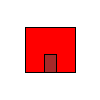
\includegraphics[width=1.2cm]{PresentationImages/body.png}
			\end{figure}		
		\end{column}
		\end{columns} 
		\begin{columns}[t]
		\begin{column}{.45\textwidth}
		\begin{verbatim}
		(scale-shape 
		  (above (overlay top bottom)) 
		1.4 1.4)

		\end{verbatim}
		\end{column}
		\begin{column}{.3\textwidth}
		\begin{figure}[h]
			
\includegraphics[width=2cm]{PresentationImages/house.png}
			\end{figure}		
		\end{column}
		\end{columns}
	\end{itemize}
	
\end{frame}

\begin{frame}[fragile]
	\frametitle{Other complex functions}
	\begin{itemize}
	\item You can orient your besides and aboves as well
	\begin{columns}[t]
		\begin{column}{.45\textwidth}
		\begin{verbatim}
(beside-align :top 
              tower 
              tight-rope 
              tower)
		\end{verbatim}
		\end{column}
		\begin{column}{.3\textwidth}
		\begin{figure}[h]
			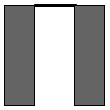
\includegraphics[width=1.22cm]{PresentationImages/towers.png}
			\end{figure}		
		\end{column}
		\end{columns} 
		\begin{columns}[t]
		\begin{column}{.45\textwidth}
		\begin{verbatim}
(above-align :right 
             block1 
             block1.3
             block1.6)
		\end{verbatim}
		\end{column}
		\begin{column}{.3\textwidth}
		\begin{figure}[h]
			
\includegraphics[width=1.1cm]{PresentationImages/left-tower.png}
			\end{figure}		
		\end{column}
		\end{columns} 
		\begin{columns}[t]
		\begin{column}{.45\textwidth}
		\begin{verbatim}
(beside-align :top 
              tower-aligned-R 
              tight-rope 
              tower-aligned-L)
		\end{verbatim}
		\end{column}
		\begin{column}{.3\textwidth}
		\begin{figure}[h]
			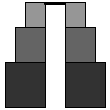
\includegraphics[width=1.5cm]{PresentationImages/two-tower.png}
			\end{figure}		
		\end{column}
		\end{columns}
	\end{itemize}
	
\end{frame}

\begin{frame}[fragile]
	\frametitle{The draw-shape function}
	\begin{itemize}
	\item Draw-shape (or ds, either work) is the function that handles taking in these shape objects and drawing the elements of them appropriately.
		\begin{verbatim}
(draw-shape 
   (create-rect 200 200 :red) 
   400 400)
		\end{verbatim}
		
		\begin{verbatim}
(draw-shape 
   (beside box1
           box2
           circle
           triangle))
		\end{verbatim}
	\end{itemize}
\end{frame}


\begin{frame}[fragile]
	\frametitle{The draw-shape function}
		\begin{verbatim}
{:w w
 :h h
 :tw w
 :th h
 :dx 0
 :dy 0
 :angle 0
 :ds (fn [x y pict wid hei cs angle]
       (*large cond to check fill/stroke here*)
       (with-translation [x y]
         (with-rotation 
           [(/ (* PI angle) 180)] 
           (f-rect 0 0 wid hei)))
       (no-fill))}
		\end{verbatim}		
\end{frame}



%Build house slides, round window

\begin{frame}
	\frametitle{Our direction}
	\begin{itemize}
		\item Less paintbrush, more collage
		%An artist finds more use in a brush while a beginner
		%isn't skilled enough
		\item Create shapes, not just draw them
		%Teach students to think about shapes without positions
		% Drawing a flower, not 9 cut ellipisies and a circle and 
		%a bunch of coordinates
		\item Easier student code
		%Not distracting from learning basic concepts
		%Works with flow of basic concepts
		\item Give students an idea of how good software should be built              
		%by giving a language like that promotes it by design
	\end{itemize}
\end{frame}

\begin{frame}
	\frametitle{A few examples}
	 Please Enjoy a Few Live Examples
\end{frame}

\begin{frame}
	\frametitle{Future work}
	\begin{itemize}
		\item Fill out more functionality
		\begin{itemize}
			\item Rotate more complex shapes
			\item Pixel-detail Overlay and Overlay-Align
			\item More seemless integration with Quil fun-mode
		\end{itemize}
		\item Open Source the project
		\item Integrate a Clojure sound library
	\end{itemize}
\end{frame}

\begin{frame}
\frametitle{Acknowledgments}
	Our research was sponsored by:
	\begin{itemize}
	\item HHMI
	\item LSAMP
	\end{itemize}
	{\centering
	\noindent
	Thank you! \par
	Any questions? \par
	}
\end{frame}
\end{document}
Status API Training Shop Blog About Help
© 2015 GitHub, Inc. Terms Privacy Security Contact
